%
% Documentation for the path openings code
%
%
% Hugues Talbot	 1 Dec 2009
%

\documentclass[11pt]{article}
\usepackage{a4wide}
\usepackage{graphicx}
\usepackage{subfigure}
\usepackage{hyperref}

\title{Path opening library}
\author{Ben Appleton and Hugues Talbot}

\begin{document}
\maketitle

\section{Introduction}
Path openings and closing~\cite{Talbot2007,Heijmans2005,Appleton2005,Heijmans2004,Buckley2000} are a way to filter an image using mathematical morphology principles~\cite{serra88,serra82}, \cite{pierres_book03},\cite{Najman2008b} using families of paths as structuring elements.

In most filtering techniques, a noise and/or an image model are assumed, e.g. Gaussian noise and piecewise smooth images. With mathematical morphology, we assume images contains objects and/or noise which conform to some geometrical and/or topological properties.

Structuring elements, which are basically sliding windows on which we compute a maximum or a minimum instead of a mean or a median, are key to this idea. Their shape and size are important. For instance, say that we want to extract (technically, to segment) thin objects that are locally linear. We could use families of straight segments, as in~\cite{Soille2001} to filter out anything that would not be locally so, and use other filters such as a top-hat to eliminate thick objects.

However, very thin objects would also be filtered out using a family of segments. Instead, it would be useful to be able to use structuring elements that are locally linear but not necessarily perfectly straight. This is where path openings come in: they allow us to use families of paths that fit within a more or less constrained cone. 

Such families have a population that grows exponentially with the path length. If we were to implement path openings by combining ``traditional'' structuring-element-based approach, it would be unworkable. 

Instead, path openings employ a decomposition technique described in~\cite{Heijmans2005} and an ordered algorithm described in~\cite{Talbot2007} to achieve very reasonable computing times. We can also improve this approach by leaving a few pixels out of the paths at random, which makes them very robust to noise.

In essence, a path opening will regain any bright feature over a darker background in which a path of a given length can fit. A path closing does the same for dark features over a bright background.

\begin{figure}
\centering
\subfigure[]{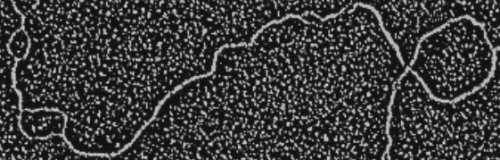
\includegraphics[width=0.8\textwidth]{DNAGI.png}}\\
\subfigure[]{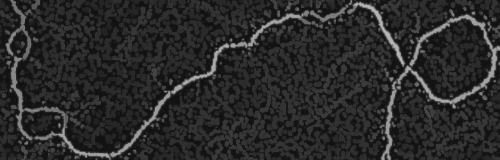
\includegraphics[width=0.8\textwidth]{DNAGI_70_3.png}}
\caption{Example path opening with length 70 pixels and tolerance 3 : (a) original, (b) filtered result}
\end{figure}

\section{Code compilation}
Code compilation is fairly straightforward. 

\paragraph{Requirements}
The library {\sc ImageMagick} is
required, with its associated development files. For instance, under Ubuntu
10.4, the following packages are required:

\begin{itemize}
\item {\tt libmagickcore2}
\item {\tt libmagickcore-dev}
\end{itemize}

Note that ImageMagick is only required for image I/O, so if {\tt
  /usr/include/ImageMagick/magick/api.h} is installed, and the script {\tt
  MagickCore-config} is in your path, most likely you will be fine. The rest of
the distribution is self-contained.

Under Windows, try using the \url{http://www.cygwin.com/}{Cygwin}
environment. This is currently untested. Please feel free to report success.

\paragraph{Edit the makefile}
Most likely, you will need to edit the lines

\begin{verbatim}
PREFIX=/opt/local
\end{verbatim}

in the makefile. This is valid for Mac OSX with the \href{http://www.macports.org/}{MacPorts}
project installed. For Ubuntu, change this to {\tt PREFIX=/usr} and this should
be ok.

\paragraph{Compilation}
Depending on your setting, you might also need to set up the 
{\tt PKG\_CONFIG\_PATH} environment variable, if the program. The symptom is the
following:

\begin{quote}
\begin{verbatim}
Package MagickCore was not found in the pkg-config search path.
Perhaps you should add the directory containing `MagickCore.pc'
\end{verbatim}
\end{quote}

For example, you might have to type

\begin{verbatim}
export PKG_CONFIG_PATH=/opt/local/lib/pkgconfig
\end{verbatim}

Then just type {\tt make} in a terminal.

\section{Usage}
The makefile will produce an executable called {\tt test\_pathopen}

\begin{quote}
\begin{verbatim}
$ ./test_pathopen 
Usage : ./test_pathopen <input image> L K <output image>
Where : <input image> is an 8-bit grey-level image in any format readable by ImageMagick
        L is the length of the path 
        K is the number of admissible missing pixels 
        <output image> is an 8-bit image. The extention determines the format
\end{verbatim}
\end{quote}

There is an example image in the {\tt images} directory.

just run the following example:


\begin{quote}
\begin{verbatim}
./test_pathopen images/DNAGI.tif 70 1 result.tif
\end{verbatim}
\end{quote}

Any output format is suitable, just specify it by its extension ({\tt
  result.png}, etc), however make sure your output format is compatible with
16-bit output, so TIFF and PGM are good choices.

With the above parameters, the results is shown in Fig.~\ref{fig:pathopening}.

\begin{figure}
\centering
\subfigure[Initial image]{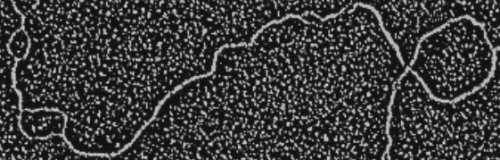
\includegraphics[width=0.8\textwidth]{DNAGI.png}}\\
\subfigure[Path opening with L=70,K=1]{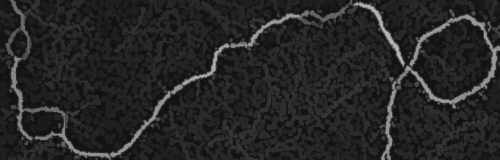
\includegraphics[width=0.8\textwidth]{DNAGI_70_1.png}}\\
\caption{Path opening result\label{fig:pathopening}}
\end{figure}


\section{Library}

Here be the documentation about the ABI.

\bibliography{pathopenings}
\bibliographystyle{plain}

\end{document}